\documentclass[11pt]{article}
\usepackage{scribe}
\usepackage{graphicx}

% Uncomment the appropriate line
%\Scribe{Your name}

\Scribes{Frendy Lio Can}
\LectureDate{February 10, 2021}
\LectureTitle{Homework 1}

%\usepackage[mathcal]{euscript}


\begin{document}

\MakeScribeTop

%\paragraph{This is a paragraph heading} Paragraph.

%%%%%%%%%%%%%%%%%%%%%%%%%%%%%%%%
% PROBLEM 1
%%%%%%%%%%%%%%%%%%%%%%%%%%%%%%%%
\paragraph{\noindent\textbf{\LARGE{Problem B.1}}}

% Start of Explaining

\begin{flushleft}
    a) $AMAT = cache_{hit} + cache_{miss} = 97\% * 1 + 3\% * 110 = 4.27$ cycles.
    \newline
    
    b) $Hit_{rate} = \frac{64 KB}{1 GB} = 0.000064$ 
    \newline
    $AMAT = cache_{hit} + cache_{miss} = 0.000064 * 1 + (1 - 0.000064) * 110 = 109.99$ cycles.
    \newline

    c) The cache memory would be of not use as when the cache is disabled the cycles are 105 which is lower than 109.99 (from problem b).
    \newline

    d) Let Memory Access Time with no cache be, $T_{off}$; with cache, $T_{on}$; miss rate, $m_{rate}$.
    \newline
    \newline
    Therefore,
    \newline
    $T_{on} = (1 - miss_{rate})(T_{off} - G) + miss_{rate}(T_{off + L})$.
    \newline
    \newline
    We also know that cache is not useful when,
    \newline
    $T_{off}  \leq (1 - miss_{rate})(T_{off} - G) + miss_{rate}(T_{off + L})$.
    \newline
    $miss_{rate} \geq \frac{G}{G+L} \geq \frac{104}{109} \approx 0.95$
    \newline
    Therefore, the highest miss rate after the cache use would be disadvantageous is 95\%.
\end{flushleft}   


%%%%%%%%%%%%%%%%%%%%%%%%%%%%%%%%
% PROBLEM 2
%%%%%%%%%%%%%%%%%%%%%%%%%%%%%%%%
\paragraph{\noindent\textbf{\LARGE{Problem B.8}}}

% Start of Explaining

\begin{flushleft}
    a) Assuming the misses are not overlapped in memory, this imply that their effects will be accumulated. Therefore, it will take $4*100 = 400$ cycles.
    \newline

    b) Since the cache line size is 16 bytes, then every 4 iteration will mess elements a,b,c, and d.
    Thus, in average number of cycles an average iteration will take is $\frac{400}{4} = 100$ cycles.
    \newline
    
    c) Same as b), instead it will be every 16 iteration. Thus, in average number of cycles an average iteration will take is $\frac{400}{16} = 25$ cycles.
    \newline

    d) If the cache is direct-mapped and its size is reduced to 2048 bytes. It will make every array access to be a miss. This is true because for each $a_i , b_i, c_i$ and $d_i$ will map to the same cache line.
    This implies that every iteration will have 3 read misses ($a_i, b_i, c_i$) and 1 write miss ($d_i$). Beside this, we know that there will be a cost of a write back for $d_i$ that 
    goes from iteration 1 through 511.
    \newline
    Therefore, the average number of cycles is $(4 + \frac{511}{512} )* 100$
\end{flushleft}   

%%%%%%%%%%%%%%%%%%%%%%%%%%%%%%%%
% PROBLEM 3
%%%%%%%%%%%%%%%%%%%%%%%%%%%%%%%%
\paragraph{\noindent\textbf{\LARGE{Problem B.12}}}

% Start of Explaining

\begin{flushleft}
    a) Let $AMAT_{direct}$ be the direct-mapped cache; $\text{AMAT}_{associative}$ the 4-way associative cache; and, $m_i$ the miss rate of a cache. Therefore, if the miss penalty is $100ns$ we can conclude the following.
    \newline
    $\text{AMAT}_{direct} = 0.22 + 100 *m_1$
    \newline
    $\text{AMAT}_{associative} = 0.52 + 100*m_2$
    \newline

    Thus, it will be advantageous to use the smaller cache when:
    \newline
    $\text{AMAT}_{direct} \leq \text{AMAT}_{associative}$
    \newline
    $0.22 + 100 *m_1 \leq  0.52 + 100*m_2$
    \newline
    $m_1 \leq 0.003 + m_2$
    \newline

    b) We know that $\text{AMAT} = \text{Hit time} = \text{Miss Rate} * \text{Miss Penalty}$, where $\text{Miss Penalty} = \text{Hit Time * Cycles}$. Therefore,
    \newline
    Miss penalty of $10$: $m_1 \leq 0.136 + 2.364m_2$
    \newline
    Miss penalty of $1000$: $m_1 \leq 0.0136 + 2.364m_2$
    \newline
    \newline
    Thus, you should use a smaller cache when the data being cache is small.
\end{flushleft}   


%%%%%%%%%%%%%%%%%%%%%%%%%%%%%%%%
% PROBLEM 4
%%%%%%%%%%%%%%%%%%%%%%%%%%%%%%%%
\paragraph{\noindent\textbf{\LARGE{Problem C.1}}}

% Start of Explaining

\begin{flushleft}
    a)
    \newline
    \begin{center}
    \begin{tabular}{ | m{10em} | m{10em}| m{10em} | } 
        \hline
        Register & Line \#s of the instructions & Type of data dependencies, e.g., RAW, WAR, WAW \\ 
        \hline
        x1 & 1,2 & RAW \\ 
        \hline
        x1 & 1,2 & WAW \\ 
        \hline
        x2 & 4,5   & RAW \\
        \hline
        x4 & 5, 6 & RAW \\
        \hline
    \end{tabular}
    \end{center}

    b)
    \newline

    \begin{figure}[htbp]
        \centerline{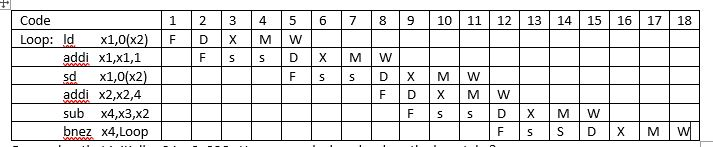
\includegraphics[scale=1]{Capture.JPG}}
        \label{fig}
    \end{figure}

    The loop takes 1586 cycles. 
    \newline
    We know that $x_3 = x_2 + 396$ which implies that the loop will run $\frac{396}{4} = 99$ times. We also know that due to flushing, the loop will take 16 cycles. We also know that the last loop will run 18 cycles.
    Therefore, the total of cycles is $98*16 + 18 = 1586$.
\end{flushleft}   

%%%%%%%%%%%%%%%%%%%%%%%%%%%%%%%%
% PROBLEM 5
%%%%%%%%%%%%%%%%%%%%%%%%%%%%%%%%
\paragraph{\noindent\textbf{\LARGE{Problem C.3}}}

% Start of Explaining

\begin{flushleft}
    a) We know that MEM stage is the slowest, $2ns$ and the pipeline register delay is $0.1ns$. Therefore the clock cycle time is $2.1ns$.
    \newline
    \newline

    b) We know that the ideal CPI is 1. Since there is a stall every 4 instruction.
    \newline
    CPI $= 1 + \frac{1}{4} = 1.25$
    \newline

    c)
    \newline
    Speedup = $\frac{I*1*7}{I*1.25*2.1} = 2.67$.
    \newline

    d)
    \newline
    The speedup would be equal to the number of tasks/instruction
\end{flushleft}   

%%%%%%%%%%%%%%%%%%%%%%%%%%%%%%%%
% PROBLEM 6
%%%%%%%%%%%%%%%%%%%%%%%%%%%%%%%%
\paragraph{\noindent\textbf{\LARGE{Problem C.7}}}

% Start of Explaining

\begin{flushleft}
    a) 
    \newline
    Execution time of 5-stage = $I*(1+\frac{1}{5}) * 1 = 1.20I$
    \newline
    Execution time of 12-stage = $I*(1+\frac{3}{8}) * 0.6 = 0.825I$
    \newline
    Speedup $= \frac{1.25}{0.825} = 1.45$
    \newline
    \newline
    b)
    \newline
    $CPI_{5-stages} = \frac{6}{5} + 0.20*0.05*2 =  1.22 $
    \newline
    $CPI_{12-stages} = \frac{11}{8} + 0.20*0.05*5 =  1.425 $
\end{flushleft}   

\end{document}
